% Book pp. 159-165 (PDF pp. 160-166)
\section{Tangents and Normals}

\begin{center}
\textbf{\color{sectionblue} Study Figure 4.22 carefully:}
\end{center}
\begin{center}
\begin{tikzpicture}[scale=1.1]
  \coordinate (V) at (0,0);
  \coordinate (O) at (-45:1.5);
  \draw[black, thick] (V) circle (1.5);
  \draw[blue!60!black] ($(O)+(-140:2.6)$) -- ($(O)+(40:2.4)$);
  \draw[red, thick] (V) -- (O);
  \fill[red] (V) circle (1.2pt);
  \fill[red] (O) circle (1.2pt);
  \node[left] at (V) {V};
  \node[right] at (O) {O};
  \node[left] at ($(O)+(-140:2.6)$) {A};
  \node[right] at ($(O)+(40:2.4)$) {B};
\end{tikzpicture}
\end{center}
\figcaption{4.22}{Tangent of a circle}

In Figure 4.22, V is the circle's centre, $|$VO$|$ is a radius and AOB is a tangent to the
circle at O. The tangent is a line that touches the circle at only one point.

The equation of the radius, VO, or its extension is the normal to tangent, AOB.
The normal and the tangent intersect at right angles at the point of tangency.

Since $|$VO$|$ and $|$AOB$|$ intersect at right angles,

We have the (gradient of $|$OV$|$ )$\times$ (gradient of $|AOB|$) $= -1$

Let us use this relation to answer a few questions.

\subsection{How to find the equation of a tangent and normal given the circle
equation and a point, $(a, b)$, on the circumference of the circle}

\textbf{Step 1:} Using the given circle equation, find the centre, (h, k)

\textbf{Step 2:} Find the gradient of the normal. This is the gradient (m) of the line
connecting points (h, k) and (a, b)

\textbf{Step 3:} Find the gradient of the tangent. The gradient of the tangent is $-\frac{1}{m}$, where
$m$ is the gradient of the normal.

\textbf{Step 4:} Find the equation of the tangent. This is given as:
\[ y - b = -\frac{1}{m}(x - a) \]
The equation of the normal is $y - k = m(x - h)$

Where $(a, b)$ is a point on the circumference of the circle and (h, k) is the centre
of the circle.

\begin{example}{Example 4.9}
Find the equations of the line tangent and normal to the circle $x^2 + y^2 = 169$ at
point $(5, -12)$

\solution
First find the centre of the circle.

To do this, we will write the equation in the standard form:
\[ (x - 0)^2 + (y - 0)^2 = 13^2 \]
This is a circle with a centre (0, 0) and a radius of 13 units.

Next, we will check if the given point satisfies the circle equation.
\[ 5^2 + (-12)^2 = 25 + 144 = 169 \]
This shows that $(5, -12)$ is on the circumference of the circle.

Next, find the gradient of the normal. This is the gradient of the line connecting
the points (0, 0) and (5, -12)
\[ m = -\frac{12 - 0}{5 - 0} = -1\tfrac{2}{5} \]
\booknote[S4-10]{$-\frac{12}{5}$ is printed as the mixed number $-1\frac{2}{5}$; it is
$-2\frac{2}{5}$. Below, the gradient of the tangent is printed as
``$-\frac{1}{m} = -\frac{\frac{1}{12}}{5} = 1 \times \frac{5}{12} = \frac{5}{12}$''; it should
read $-\frac{1}{m} = -\dfrac{1}{-\frac{12}{5}} = 1 \times \frac{5}{12} = \frac{5}{12}$.}
Equation of the normal is: $y - 0 = -\frac{12}{5}(x - 0)$

Multiply through by 5:
\[ 5y = -12x \]
$5y + 12x = 0$ is the equation of the normal.

The gradient of the tangent is $= -\dfrac{1}{m} = -\dfrac{\frac{1}{12}}{5} = 1 \times \dfrac{5}{12} = \dfrac{5}{12}$

The equation of the tangent is: $y - (-12) = \frac{5}{12}(x - 5)$
\[ (y + 12) = \frac{5}{12}(x - 5) \]
Multiply through by 12:
\begin{align*}
12y + 144 &= 5x - 25 \\
12y - 5x + 144 + 25 &= 0
\end{align*}
$12\boldsymbol{y} - 5\boldsymbol{x} + 169 = 0$ is the equation of the tangent.
\end{example}

\begin{example}{Example 4.10}
The point (5, 3) satisfies the equation $x^2 + y^2 - 6x - 4y + 8 = 0$.
\begin{enumerate}
  \item[a.] Find the radius of the circle.
  \item[b.] Fine the equation of the normal to the circle at point (5, 3)
  \item[c.] Find the equation of the tangent to the circle at (5, 3)
\end{enumerate}

\solution
\begin{enumerate}
  \item[a.] To find the radius, write the equation in standard form
  \begin{align*}
  x^2 - 6x + 9 + y^2 - 4y + 4 &= -8 + 9 + 4 \\
  (x - 3)^2 + (y - 2)^2 &= 5 \\
  \left(x - 3\right)^2 + \left(y - 2\right)^2 &= \left(\sqrt{5}\right)^2
  \end{align*}
  This means the \textbf{radius is} $\sqrt{5}$ \textbf{and the centre is} (3, 2).

  Gradient of the normal.

  This is the gradient of the line connecting the points (3, 2) and (5, 3)
  \item[b.] The gradient of the normal $= \dfrac{3 - 2}{5 - 3} = \dfrac{1}{2}$

  The equation of the normal is: $y - 2 = \frac{1}{2}(x - 3)$
  \begin{align*}
  2y - 4 &= x - 3 \\
  2y - x - 4 + 3 &= 0 \\
  2\boldsymbol{y} - \boldsymbol{x} - 1 &= 0
  \end{align*}
  Gradient of the tangent $= -1 \div \frac{1}{2} = -2$
  \item[c.] The equation of the tangent is:
  \begin{align*}
  y - 3 &= -2(x - 5) \\
  y - 3 &= -2x + 10 \\
  \boldsymbol{y} + 2\boldsymbol{x} - 13 &= 0
  \end{align*}
\end{enumerate}
\end{example}

\begin{example}{Example 4.11}
Find the equation of the normal to the circle $y^2 + x^2 + 8x + 7 = 0$ that passes
through the point (1, 3)

\solution
First, verify if the point lies on the circumference of the circle:
\[ (3)^2 + (1)^2 + 8(1) + 7 \ne 0 \]
Therefore, the point (1, 3) is not on the circle's circumference.

Next, find the coordinates of the centre of the circle.
\begin{align*}
\text{The centre is given as} = {} & \left(\frac{\textit{coefficient of } x}{-2}, \frac{\textit{coefficient of } y}{-2}\right) \\
= {} & \left(\frac{8}{-2}, \frac{0}{-2}\right) \\
= {} & (-4, 0)
\end{align*}
The gradient of the normal $= \dfrac{-3}{-4 - 1} = \dfrac{3}{5}$

Equation of the normal: $y - 3 = \frac{3}{5}(x - 1)$
\begin{align*}
5y - 15 &= 3x - 3 \\
5y - 3x - 15 + 3 &= 0 \\
5\boldsymbol{y} - 3\boldsymbol{x} - 12 &= 0
\end{align*}
The diagram below shows the construction of the circle and the normal
\begin{center}
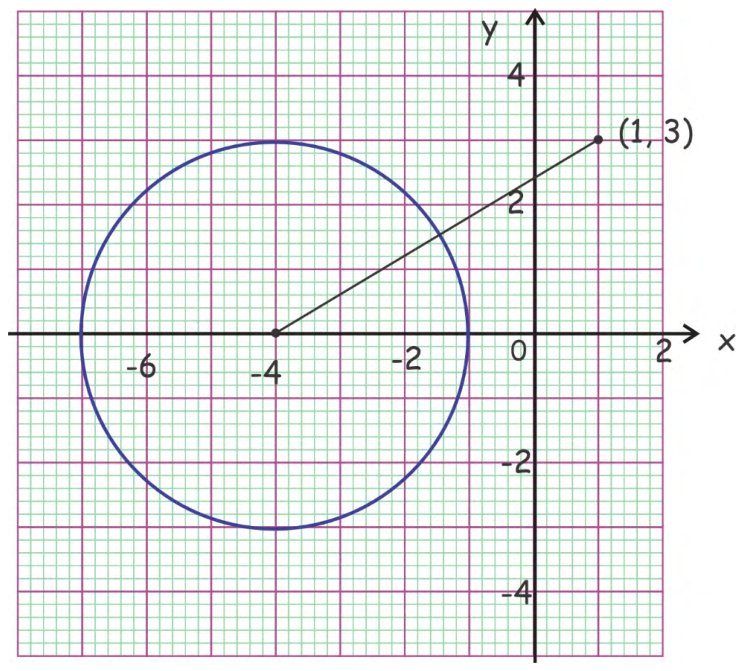
\includegraphics[width=0.6\linewidth]{figures/fig4-23.jpg}
\end{center}
\figcaption{4.23}{Construction of a circle and normal}
\end{example}

\subsection{Length of a tangent (L)}

Given the equation of a circle, it is possible to find the length of a tangent to the
circle from a point $(x, y)$ outside the circle.

Figure 4.24 illustrates this:
\begin{center}
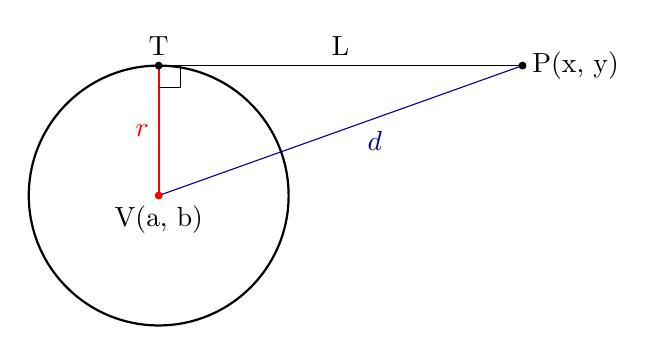
\begin{tikzpicture}[scale=1.1]
  \coordinate (V) at (0,0);
  \coordinate (T) at (0,1.5);
  \coordinate (P) at (4.2,1.5);
  \draw[black, thick] (V) circle (1.5);
  \draw[black] (T) -- (P);
  \draw[blue!60!black] (V) -- (P);
  \draw[red, thick] (V) -- (T);
  \draw (0,1.5) ++(0.25,0) -- ++(0,-0.25) -- ++(-0.25,0);
  \fill[red] (V) circle (1.3pt);
  \fill[black] (T) circle (1.3pt);
  \fill[black] (P) circle (1.3pt);
  \node[above] at (T) {T};
  \node[above] at (2.1,1.5) {L};
  \node[right] at (P) {P(x, y)};
  \node[below] at (V) {V(a, b)};
  \node[red, left] at (0,0.75) {$r$};
  \node[blue!60!black, below right] at (2.3,0.85) {$d$};
\end{tikzpicture}
\end{center}
\figcaption{4.24}{Length of a tangent}

In Figure 4.24, V(a, b) is the centre of the circle. T is a point of tangency and P($x$,
$y$) is any point outside the circle. The length of the tangent is $|$PT$| = L$.

From Pythagoras' theorem, we have $L^2 + r^2 = d^2$, since we are interested in
finding L, make it the subject.
\begin{align*}
L^2 &= d^2 - r^2 \\
\sqrt{L^2} &= \sqrt{d^2 - r^2} \\
L &= \sqrt{d^2 - r^2}
\end{align*}

\begin{example}{Example 4.12}
Find the length of the tangent from the point (0, 4) to the circle $x^2 + y^2 - 2x +
12y - 3 = 0$
\booknote[S4-11]{the circle worked in the solution (and named in the caption of
Figure 4.25) is $x^2 + y^2 - 6x + 4y - 3 = 0$, with centre $(3, -2)$ and radius 4;
the equation printed in the question does not match it. For the circle as
printed, the centre is $(1, -6)$, $r^2 = 40$, $d^2 = 101$ and the length is
$\sqrt{61}$.}

\solution
First find the centre and radius of the circle:
\begin{align*}
x^2 - 6x + 9 + y^2 + 4y + 4 - 3 &= 9 + 4 \\
(x - 3)^2 + (y + 2)^2 &= 16 \\
(x - 3)^2 + (y + 2)^2 &= 4^2
\end{align*}
The centre of the circle is (3, -2) and the radius is 4
\begin{center}
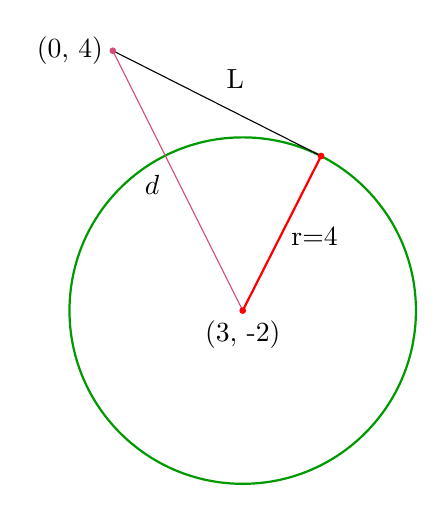
\begin{tikzpicture}[scale=0.55]
  \coordinate (C) at (3,-2);
  \coordinate (P) at (0,4);
  \coordinate (T) at (4.81,1.57);
  \draw[green!60!black, thick] (C) circle (4);
  \draw[purple!70] (C) -- (P);
  \draw[black] (P) -- (T);
  \draw[red, thick] (C) -- (T);
  \fill[purple!70] (P) circle (2.2pt);
  \fill[red] (C) circle (2.2pt);
  \fill[red] (T) circle (2.2pt);
  \node[left] at (P) {(0, 4)};
  \node[below] at (C) {(3, -2)};
  \node[above right] at (2.4,2.9) {L};
  \node[left] at (1.3,0.9) {$d$};
  \node[right] at (3.9,-0.3) {r=4};
\end{tikzpicture}
\end{center}
\figcaption{4.25}{Length of the tangent to the circle $x^2 + y^2 - 2x + 12y - 3 = 0$}

Distance between the (0, 4) and the centre (3, -2), $d = \sqrt{(3 - 0)^2 + (-2 - 4)^2}$
\begin{align*}
d &= \sqrt{(3)^2 + (-6)^2} \\
d &= \sqrt{9 + 36} \\
d &= \sqrt{45}
\end{align*}
Length of the tangent $= \sqrt{d^2 - r^2}$
\begin{align*}
\text{Length of the tangent} &= \sqrt{\left(\sqrt{45}\right)^2 - (4)^2} \\
&= \sqrt{45 - 16} \\
&= \sqrt{29}
\end{align*}
\end{example}

\begin{example}{Example 4.13}
Figure 4.26 shows a graph of a circle. Line OBA is a tangent to the circle at B.
\begin{center}
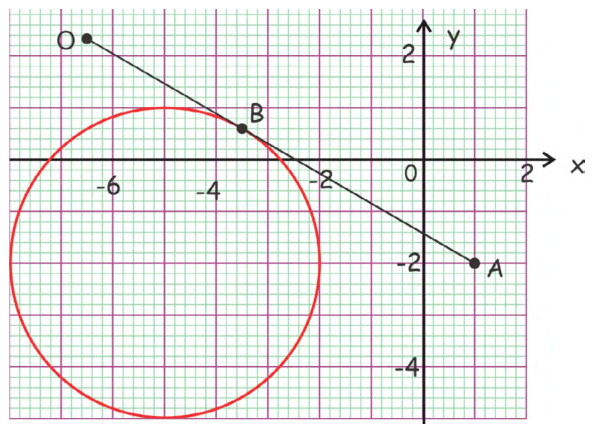
\includegraphics[width=0.5\linewidth]{figures/fig4-26.png}
\end{center}
\figcaption{4.26}{Graph of a circle with Line OBA as tangent}
\begin{enumerate}
  \item[a.] Find the equation of the circle.
  \item[b.] Find $|$AB$|$, leave your answer in surds
\end{enumerate}

\solution
\begin{enumerate}
  \item[a.] The centre of the circle is (-5, -2) and the radius is 3.
  \begin{center}
  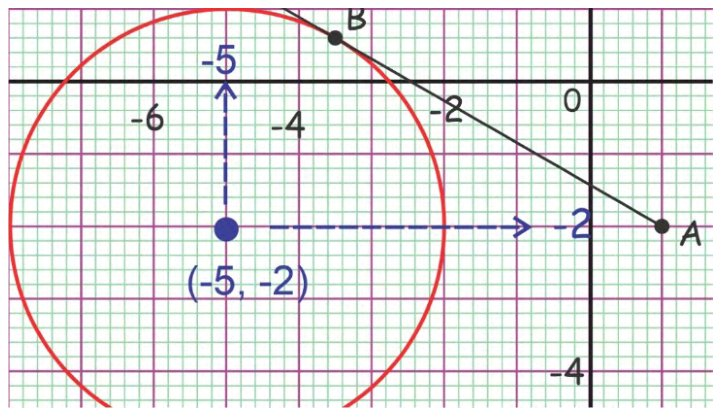
\includegraphics[width=0.6\linewidth]{figures/fig4-27.jpg}
  \end{center}
  \figcaption{4.27}{Graph of a circle with Line OBA as tangent}

  The equation of the circle is: $(x - (-5)^2 + (y - (-2))^2 = 3^2$
  \booknote[S4-12]{a bracket is missing: $(x - (-5))^2$.}
  \begin{align*}
  (x + 5)^2 + (y + 2)^2 &= 9 \\
  x^2 + 10x + 25 + y^2 + 4y + 4 - 9 &= 0 \\
  \boldsymbol{x^2 + y^2 + 10x + 4y - 5} &= \boldsymbol{0}
  \end{align*}
  \item[b.] Coordinates of point A is (1, -2)

  Distance between point A and the centre (-5, -2), $d = \sqrt{(-5 - 1)^2 + (-2 - (-2))^2}$
  \begin{align*}
  d &= \sqrt{(-6)^2 + (0)^2} \\
  d &= \sqrt{36} = 6 \\
  d &= 6
  \end{align*}
  Length of the tangent $= \sqrt{6^2 - 3^2} = \sqrt{36 - 6} = \sqrt{30}$
  \booknote[S4-13]{$3^2 = 9$, not 6: the length is $\sqrt{36 - 9} = \sqrt{27} = 3\sqrt{3}$.}
\end{enumerate}
\end{example}
